\documentclass{beamer}

\usepackage[utf8]{inputenc}
\usepackage{listings}
\usepackage{caption}
\captionsetup[figure]{font=tiny}

\usetheme{Copenhagen}
\setbeamertemplate{navigation symbols}{}
\setbeamertemplate{headline}{}
\setbeamertemplate{footline}{}

\title{Invariant and Equivariant Neural Networks}
\author[Adrian Salewsky]{Adrian Salewsky}
\institute{Technische Universität Berlin}
\date{12.05.2023}

\begin{document}

\frame{\titlepage}


\section{Introduction} 
\begin{frame}
\frametitle{Introduction}
\begin{figure}[h]
\centering{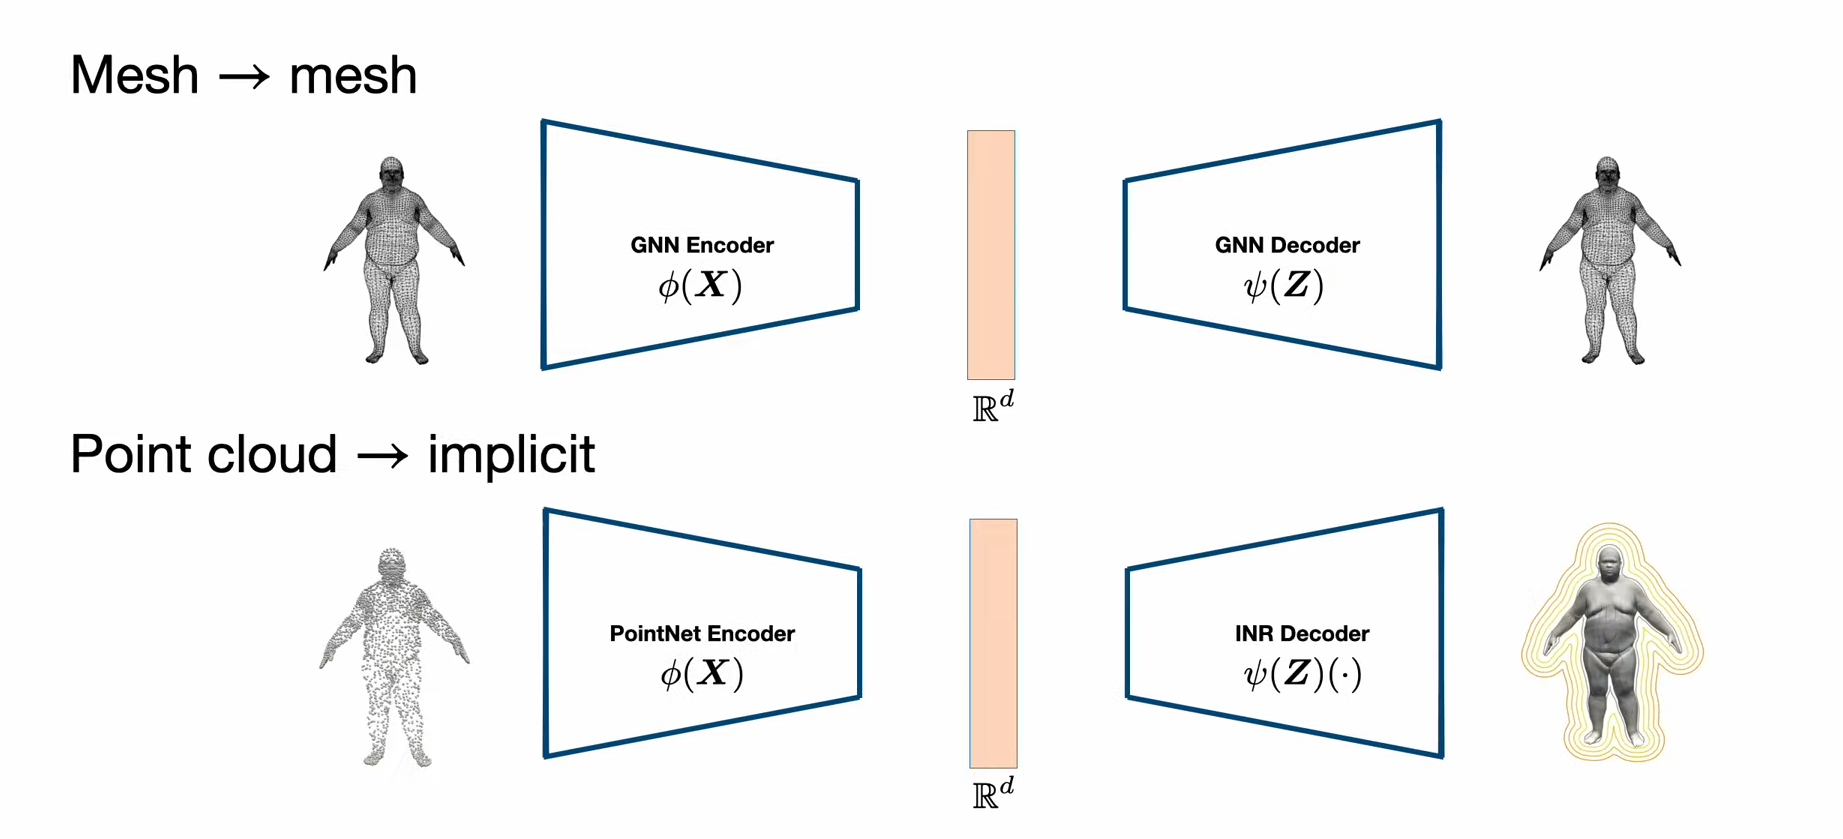
\includegraphics[scale=.25]{images/encoder-decoder}}
\caption{https://www.youtube.com/watch?v=Lft6r5oVyXM}
\end{figure}
\end{frame}

\section{Invariance and Equivariance}
\begin{frame}
\frametitle{Invariance}
\begin{figure}[h]
\centering{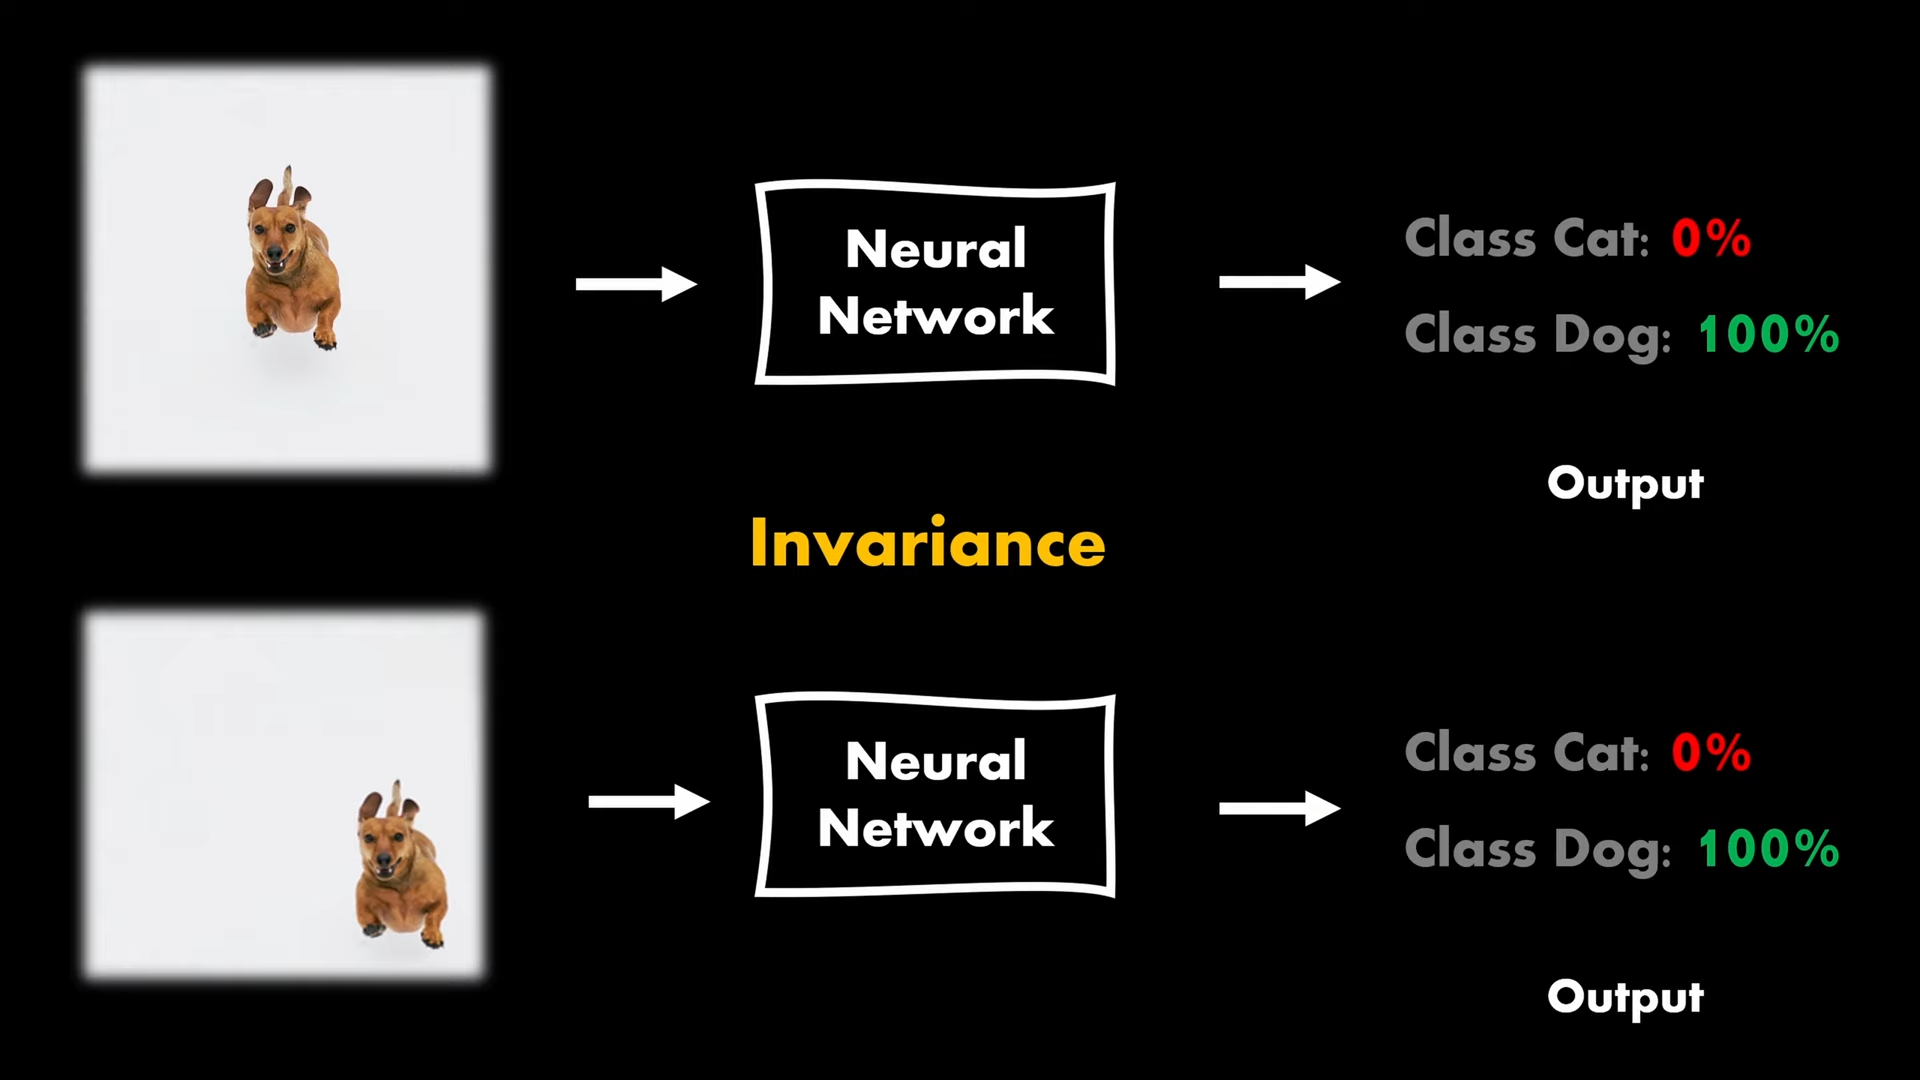
\includegraphics[scale=.2]{images/invariance}}
\caption{https://www.youtube.com/watch?v=2bP\_KuBrXSc}
\end{figure}
\end{frame}

\begin{frame}
\frametitle{Equivariance}
\begin{figure}[h]
\centering{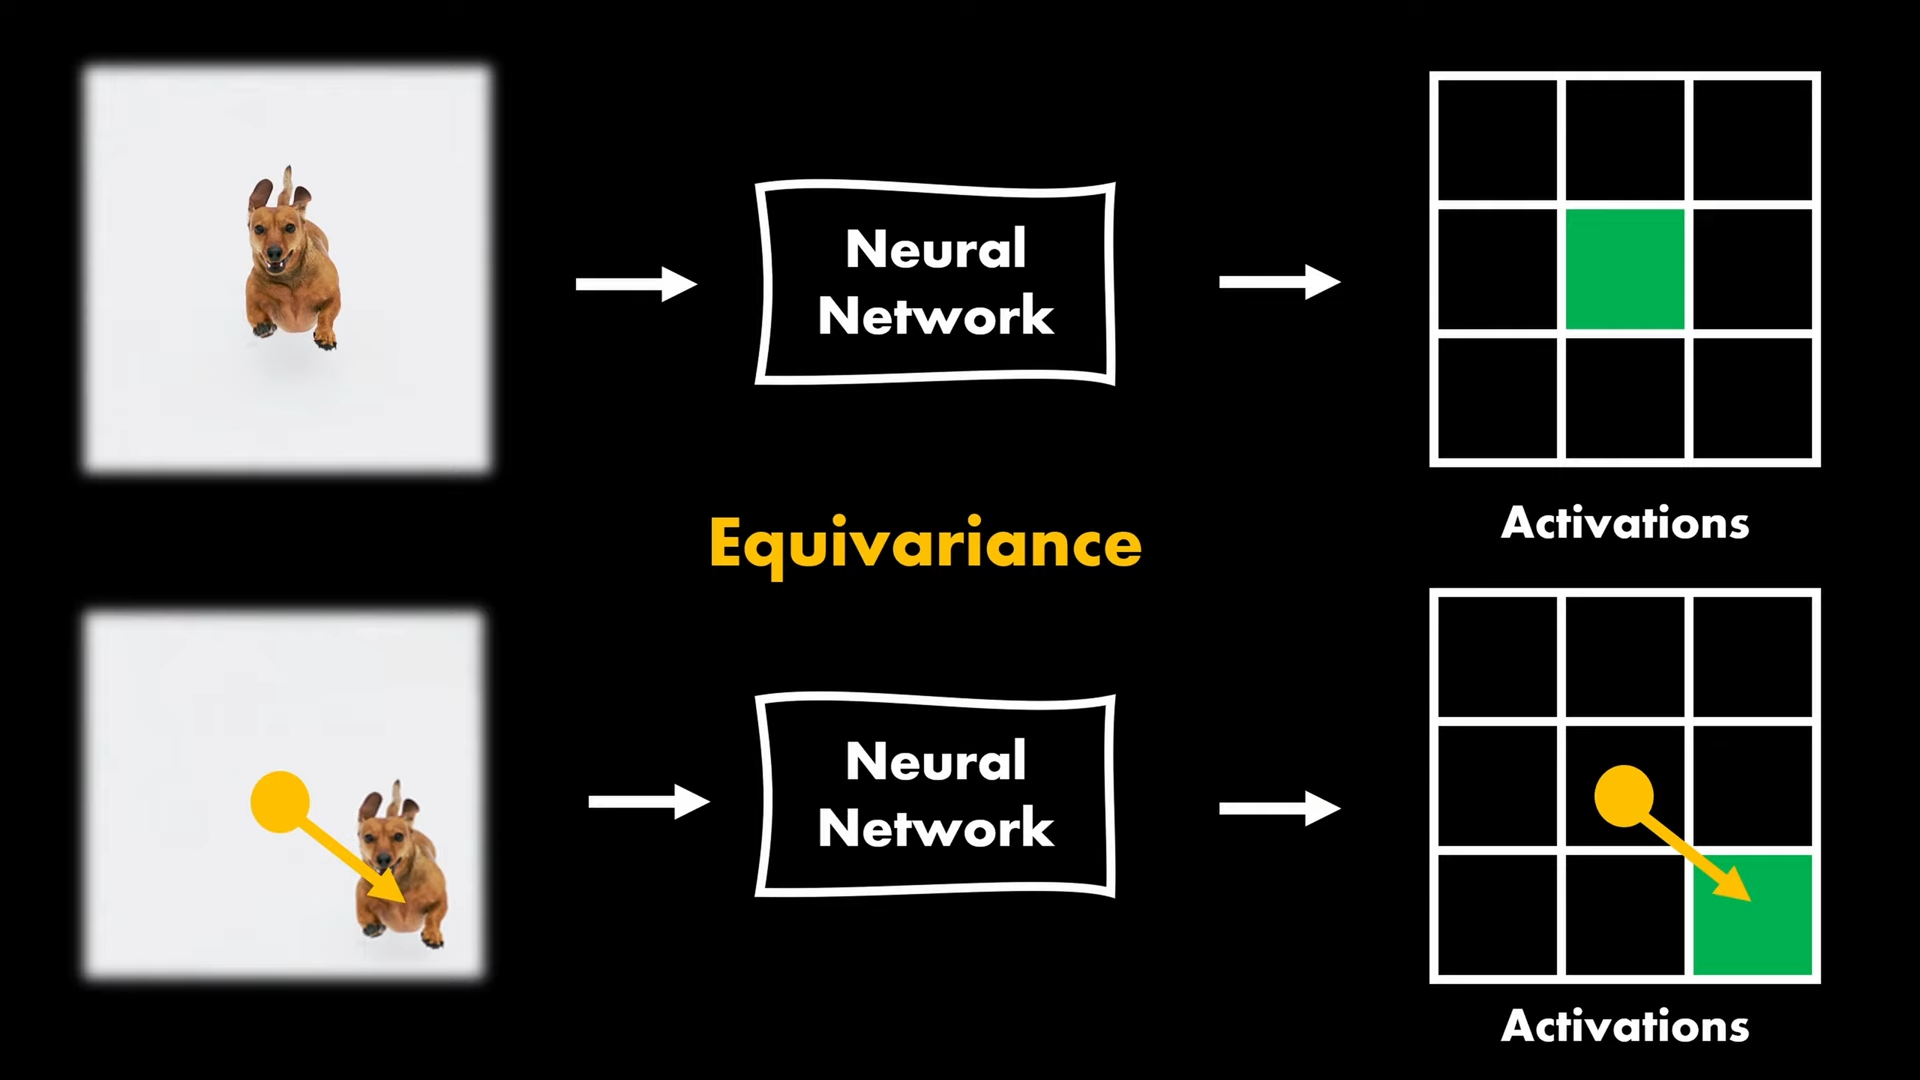
\includegraphics[scale=.2]{images/equivariance}}
\caption{https://www.youtube.com/watch?v=2bP\_KuBrXSc}
\end{figure}
\end{frame}


\section{Frame Averaging}
\begin{frame}
\frametitle{Frame Averaging}
\begin{itemize}
\item<2-> Group averaging is needed to make functions invariant/equivariant
\bigskip
\item<3-> Groups can be infinite (e.g. E(3)) $\rightarrow$ complete averaging is impossible
\bigskip
\item<4-> Instead find function (called frame) that assigns to subgroup of a group
\bigskip
\item<5-> If frame invariant/equivariant $\rightarrow$ only averaging over frame needed
\end{itemize}
\end{frame}

\section{Outlook}
\begin{frame}
\frametitle{Outlook}
\begin{itemize}
\item<2-> Implement Autoencoder for Mesh $\rightarrow$ Mesh 
\bigskip
\item<3-> Introduce layer-wise equivariance in decoder part
\bigskip
\item<4-> Layer-wise results could contain learnable features (e.g. DatasetGAN)
\bigskip
\item<5-> FAUST Dataset
\end{itemize}
\end{frame}

\end{document}